\documentclass[tikz, border=2pt]{standalone}
\usetikzlibrary{calc, positioning, arrows.meta}

\begin{document}
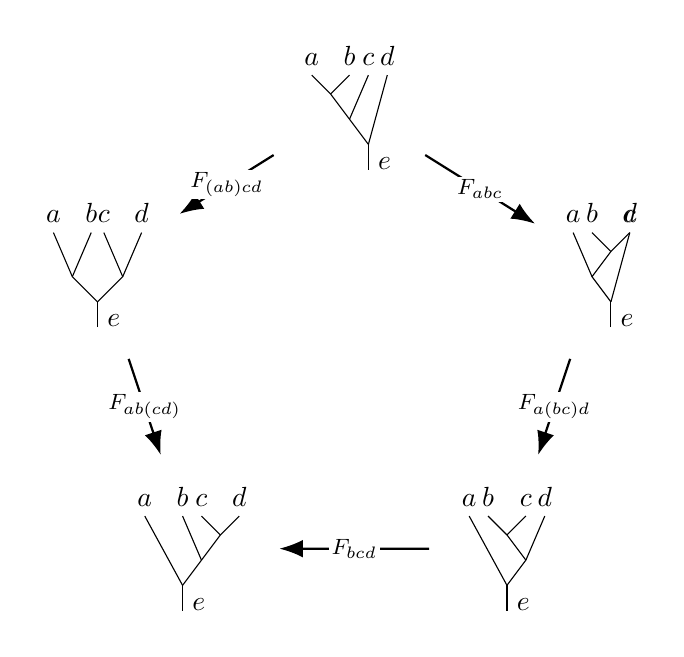
\begin{tikzpicture}[
    thick, 
    scale=0.8, 
    node distance=2cm,
    tree/.style={scale=0.4, yshift=-0.5cm},
    arrow_label/.style={midway, fill=white, font=\footnotesize, inner sep=1pt}
]

    % Define the 5 trees as pics
    
    % Tree 1: ((ab)c)d
    \tikzset{
        pics/tree1/.style={
            code={
                \draw (0,0) -- (0,0.8); % e
                \draw (0,0.8) -- (-0.6,1.6); % (ab)c
                \draw (0,0.8) -- (0.6,3); % d
                \draw (-0.6,1.6) -- (-1.2,2.4); % ab
                \draw (-0.6,1.6) -- (0,3); % c
                \draw (-1.2,2.4) -- (-1.8,3); % a
                \draw (-1.2,2.4) -- (-0.6,3); % b
                % Labels
                \node[above] at (-1.8,3) {$a$};
                \node[above] at (-0.6,3) {$b$};
                \node[above] at (0,3) {$c$};
                \node[above] at (0.6,3) {$d$};
                \node[right] at (0,0.2) {$e$};
            }
        }
    }
    
    % Tree 2: (a(bc))d
    \tikzset{
        pics/tree2/.style={
            code={
                \draw (0,0) -- (0,0.8);
                \draw (0,0.8) -- (-0.6,1.6);
                \draw (0,0.8) -- (0.6,3); % d
                \draw (-0.6,1.6) -- (-1.2,3); % a
                \draw (-0.6,1.6) -- (0,2.4); % bc
                \draw (0,2.4) -- (-0.6,3); % b
                \draw (0,2.4) -- (0.6,3); % c
                 % Labels
                \node[above] at (-1.2,3) {$a$};
                \node[above] at (-0.6,3) {$b$};
                \node[above] at (0.6,3) {$c$};
                \node[above] at (0.6,3) {$d$}; % Wait, rightmost
                \node[right] at (0,0.2) {$e$};
            }
        }
    }
    
    % Tree 3: a((bc)d)
    \tikzset{
        pics/tree3/.style={
            code={
                \draw (0,0) -- (0,0.8);
                \draw (0,0.8) -- (-1.2,3); % a
                \draw (0,0.8) -- (0.6,1.6); % (bc)d
                \draw (0.6,1.6) -- (0,2.4); % bc
                \draw (0.6,1.6) -- (1.2,3); % d
                \draw (0,2.4) -- (-0.6,3); % b
                \draw (0,2.4) -- (0.6,3); % c
                 % Labels
                \node[above] at (-1.2,3) {$a$};
                \node[above] at (-0.6,3) {$b$};
                \node[above] at (0.6,3) {$c$};
                \node[above] at (1.2,3) {$d$};
                \node[right] at (0,0.2) {$e$};
            }
        }
    }
    
    % Tree 4: a(b(cd))
    \tikzset{
        pics/tree4/.style={
            code={
                \draw (0,0) -- (0,0.8);
                \draw (0,0.8) -- (-1.2,3); % a
                \draw (0,0.8) -- (0.6,1.6); % b(cd)
                \draw (0.6,1.6) -- (0,3); % b
                \draw (0.6,1.6) -- (1.2,2.4); % cd
                \draw (1.2,2.4) -- (0.6,3); % c
                \draw (1.2,2.4) -- (1.8,3); % d
                 % Labels
                \node[above] at (-1.2,3) {$a$};
                \node[above] at (0,3) {$b$};
                \node[above] at (0.6,3) {$c$};
                \node[above] at (1.8,3) {$d$};
                \node[right] at (0,0.2) {$e$};
            }
        }
    }
    
    % Tree 5: (ab)(cd)
    \tikzset{
        pics/tree5/.style={
            code={
                \draw (0,0) -- (0,0.8);
                \draw (0,0.8) -- (-0.8,1.6); % ab
                \draw (0,0.8) -- (0.8,1.6); % cd
                \draw (-0.8,1.6) -- (-1.4,3); % a
                \draw (-0.8,1.6) -- (-0.2,3); % b
                \draw (0.8,1.6) -- (0.2,3); % c
                \draw (0.8,1.6) -- (1.4,3); % d
                 % Labels
                \node[above] at (-1.4,3) {$a$};
                \node[above] at (-0.2,3) {$b$};
                \node[above] at (0.2,3) {$c$};
                \node[above] at (1.4,3) {$d$};
                \node[right] at (0,0.2) {$e$};
            }
        }
    }

    % Nodes
    \node (top) at (0, 4) {\tikz\pic[tree]{tree1};};
    \node (tr) at (4, 1.5) {\tikz\pic[tree]{tree2};};
    \node (br) at (2.5, -3) {\tikz\pic[tree]{tree3};};
    \node (bl) at (-2.5, -3) {\tikz\pic[tree]{tree4};};
    \node (tl) at (-4, 1.5) {\tikz\pic[tree]{tree5};};
    
    % Arrows
    % Top -> TR: ((ab)c)d -> (a(bc))d via F_{abc}
    \draw[-{Latex[length=3mm]}, shorten >=5pt, shorten <=5pt] (top) -- (tr) node[arrow_label] {$F_{abc}$};
    
    % TR -> BR: (a(bc))d -> a((bc)d) via F_{a(bc)d}
    \draw[-{Latex[length=3mm]}, shorten >=5pt, shorten <=5pt] (tr) -- (br) node[arrow_label] {$F_{a(bc)d}$};
    
    % BR -> BL: a((bc)d) -> a(b(cd)) via F_{bcd}
    \draw[-{Latex[length=3mm]}, shorten >=5pt, shorten <=5pt] (br) -- (bl) node[arrow_label] {$F_{bcd}$};
    
    % Top -> TL: ((ab)c)d -> (ab)(cd) via F_{(ab)cd}
    \draw[-{Latex[length=3mm]}, shorten >=5pt, shorten <=5pt] (top) -- (tl) node[arrow_label] {$F_{(ab)cd}$}; 
    
    % TL -> BL: (ab)(cd) -> a(b(cd)) via F_{ab(cd)}
    \draw[-{Latex[length=3mm]}, shorten >=5pt, shorten <=5pt] (tl) -- (bl) node[arrow_label] {$F_{ab(cd)}$};

\end{tikzpicture}
\end{document}
